Targeted users are users who would use Magpie as a tool for their work. We interviewed 3 individuals who fit this criteria.\\ \\
Usability test sessions took the following format:
\begin{enumerate}
    \item Getting to know
    \item Introduction of Magpie
    \item Exploring Magpie + Discussion
    \item Satisfaction survey + End of session
\end{enumerate}
Getting to know the professional user is the first step. It is relevant to the session because it helps inform the type of targeted user they are, their knowledge of technology, their experience using amenity data, the tools they have used and their perspective regarding amenities.

\subsubsection{User 7 - Bryan Boyle}
Bryan Boyle is a lecturer at the University of Cork in Occupational sciences and Therapy.\\ With a doctorate in computer science and occupational therapy, they have published several papers related to inclusivity in public spaces (\cite{bryanboyleplaygroundinclusion2023}), and the role of technology in the lives of individuals with disabilities (\cite{bryanboylechildrenautism2022}).\\ \\
They left their contact in the market research survey. They are categorized as a \emph{targeted user} because they use amenity data for their work, and Magpie could potentially be a tool they use.\\ \\

\noindent Firstly, we got to know Bryan Boyle, his professional experience and the amenity data he uses for his work. He is mostly into research and therefore looks for datasets related to PHD topics of child development and inclusivity.
%bryan amenity info
\begin{figure}[h!]
    \centering
    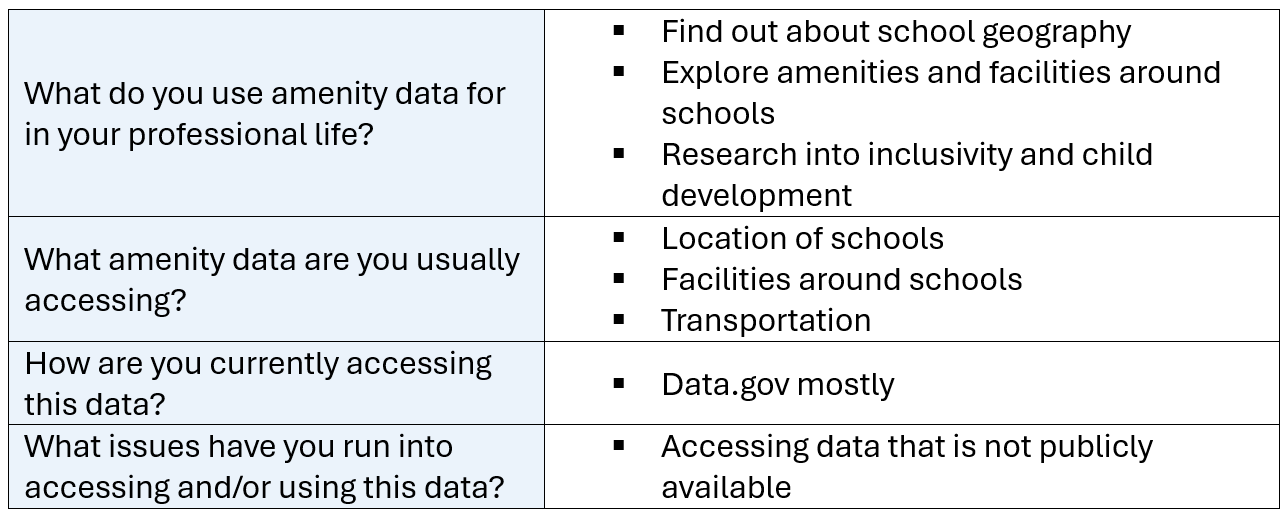
\includegraphics[width=0.7\textwidth]{images/bryan-amenity-info.png}
    \caption{User Evaluation - Bryan Boyle Information}
\end{figure}\\


\newpage
\subsubsection{User 8 - Anonymous}
Professional user Sarah

\newpage
\subsubsection{User 9 - Anonymous}
Professional user Odran